\documentclass[12pt,spanish,fleqn,openany,letterpaper,pagesize]{scrbook}

\usepackage[utf8]{inputenc}
\usepackage[spanish]{babel}
\usepackage{fancyhdr}
\usepackage{epsfig}
\usepackage{epic}
\usepackage{eepic}
\usepackage{amsmath}
\usepackage{threeparttable}
\usepackage{amscd}
\usepackage{here}
\usepackage{graphicx}
\usepackage{lscape}
\usepackage{tabularx}
\usepackage{subfigure}
\usepackage{longtable}


\usepackage{rotating} %Para rotar texto, objetos y tablas seite. No se ve en DVI solo en PS. Seite 328 Hundebuch
                        %se usa junto con \rotate, \sidewidestable ....


\renewcommand{\theequation}{\thechapter-\arabic{equation}}
\renewcommand{\thefigure}{\textbf{\thechapter-\arabic{figure}}}
\renewcommand{\thetable}{\textbf{\thechapter-\arabic{table}}}


\pagestyle{fancyplain}%\addtolength{\headwidth}{\marginparwidth}
\textheight22.5cm \topmargin0cm \textwidth16.5cm
\oddsidemargin0.5cm \evensidemargin-0.5cm%
\renewcommand{\chaptermark}[1]{\markboth{\thechapter\; #1}{}}
\renewcommand{\sectionmark}[1]{\markright{\thesection\; #1}}
\lhead[\fancyplain{}{\thepage}]{\fancyplain{}{\rightmark}}
\rhead[\fancyplain{}{\leftmark}]{\fancyplain{}{\thepage}}
\fancyfoot{}
\thispagestyle{fancy}%


\addtolength{\headwidth}{0cm}
\unitlength1mm %Define la unidad LE para Figuras
\mathindent0cm %Define la distancia de las formulas al texto,  fleqn las descentra
\marginparwidth0cm
\parindent0cm %Define la distancia de la primera linea de un parrafo a la margen

%Para tablas,  redefine el backschlash en tablas donde se define la posici\'{o}n del texto en las
%casillas (con \centering \raggedright o \raggedleft)
\newcommand{\PreserveBackslash}[1]{\let\temp=\\#1\let\\=\temp}
\let\PBS=\PreserveBackslash

%Espacio entre lineas
\renewcommand{\baselinestretch}{1.1}

%Neuer Befehl f\"{u}r die Tabelle Eigenschaften der Aktivkohlen
\newcommand{\arr}[1]{\raisebox{1.5ex}[0cm][0cm]{#1}}

%Neue Kommandos
\usepackage{Befehle}


%Trennungsliste
\hyphenation {Reaktor-ab-me-ssun-gen Gas-zu-sa-mmen-set-zung
Raum-gesch-win-dig-keit Durch-fluss Stick-stoff-gemisch
Ad-sorp-tions-tem-pe-ra-tur Klein-schmidt
Kohlen-stoff-Mole-kular-siebe Py-rolysat-aus-beu-te
Trans-port-vor-gan-ge}

\begin{document}

\section{Machine Learning}

El Aprendizaje Automático (ML) es un enfoque empírico efectivo para
regresiones y/o clasificaciones de sistemas no-lineales que pueden involucrar desde
unos pocos hasta varios cientos de variables. El enfoque de ML requiere
entrenamiento utilizando un conjunto de datos que sea representativo del conjunto
de datos del problema. Se debe seleccionar un conjunto de datos que se utilizará,
luego del entrenamiento del modelo, para validación del mismo.
ML es ideal para aquellos problemas en donde el conocimiento teórico del mismo
es incompleto o insuficiente, pero se cuenta con un gran conjunto de observaciones.
ML ha mostrado ser de utilidad para un gran número de aplicaciones en Geociencias
relacionadas a la tierra, oceanos y atmósfera, y en algoritmos de extracción
de información bio-geofísica.
Algunos de los algoritmos de ML más usados en aplicaciones relativas a
Geociencias y Sensado Remoto (GRS) son las Redes Neuronales Artificiales (ANN),
Support Vector Machines (SVM), Mapas Auto-organizados (SOM), Árboles de Decisión (DT),
Random Forests y Algoritmos Genéticos. Su aplicación en problemas de GRS es
relativamente nuevo y extremádamente prometedora. En particular, ANNs son
usadas para clasifición pero también son usadas para la aplicación en pronósticos
relativos a series de tiempo.
De hecho, una exploración en la base bibliográfica Scopus devuelve más de 4000
publicaciones que incluyen \textit{remote sensing} y \textit{neural network},
311 de ellas en 2016. De ese total, el 45\% corresponde a
\textit{Sciences of the Earth}, el 44\% a \textit{Computer Science} y el 35\% a
\textit{Engineering}; con China, Estados Unidos, Italia e India como los paises
con mayor producción científica en dichas áreas.


\subsection{Scikit-learn}
Éste proyecto inició en el 2007 como un proyecto del Google Summer Scool por David
Cournapeau. Más tarde ese año, Matthieu Brucher comenzó a trabajar en éste proyecto
como parte de su tesis. En 2010 Fabian Pedrafosa, Gael Varoquaux, Alexandre
Gramfort y Vincent Michel del INRIA \footnote{Institut National de Recherche
en Informatique et en Automatique} tomaron el liderazgo del proyecto y lo liberaron
al público por primera vez, el 1ro de Febrero de 2010. Desde entonces, salieron muchos
\textit{releases} siguiendo ciclos de 3 meses, y una gran comunidad internacional
ha estado liderando el desarrollo desde entonces.

Scikit-learn es un módulo de Python de libre acceso para Aprendizaje Automático
construido sobre \textit{SciPy}\footnote{AGREGAR QUÉ ES}. Es una herramienta
sencilla y efectiva para minería de datos y análisis de datos. Dado que está bajo
licencia BSD\footnote{PONER QUÉ ES}, esta librería puede ser utilizada tanto
para uso personal como comercial.

Con scikit-learn, los usuarios pueden realizar una gran variedad de tareas
que van desde selección de modelos, clustering, y preprocesamiento entre otras.
La librería provee un completo conjunto de tareas que permiten una
implementación completa de la solución de un problema
de Aprendizaje Automático.

Scikit-learn tiene una muy extensiva utilización. Se está utilizando por
grandes compañias en diferentes industrias desde streaming de música, hasta
recomendadores de hoteles, entre otras. Esto da la pauta de que los usuarios pueden
integrar algoritmos implementados con este módulo a sus propias aplicaciones.

Otra de las grandes bondades de la herramienta es que se asegura que tanto usuarios
antiguos como nuevos puedan obtener la asistencia que necesitan para integrar
el módulo de Aprendizaje Automático a sus propias plataformas. Ésta es la razón
que justifica el alto nivel de detalle en su documentación oficial.



\subsection{Métodos Lineales}

\subsubsection{Regresión lineal utilizando el método ordinario de Mínimos Cuadrados}

\subsubsection{Regresión lineal utilizando el método Ridge}


\subsection{Árboles de Decisión}
Los Árboles de Decisión (DTs) son métodos no paramétricos de aprendizaje supervisado
utilizados tanto para problemas de clasificación como de regresión.
La meta es crear un modelo que prediga el valor de una variable objetivo aprendiendo
simples reglas de desición inferidas a partir de las características de los datos
de entrenamientos.

El algoritmo de Árbol de Decisión construye modelos de clasificación o regresión
utilizando una estructura arbórea. Éste divide el conjunto de datos en pequeños
subconjuntos mientras que, al mismo tiempo, un árbol de decisión es incrementalmente
construido. El resultado final es un árbol con nodos de decisión y nodos hojas.
Un nodo de decisión tiene dos o más ramas, cada una representando valores para
el atributo examinado. Un nodo hoja representa una decisión dentro del
objetivo numérico. Los árboles de decisión pueden manejar tanto datos
categóricos como numéricos.

Más formalmente, dados los vectores de entrenamiento $x_{i} \in R^{n}$, $i = 1,..,l$
y un vector de etiquetas $y \in R^{l}$, un árbol de decisión particiona
recursivamente el espacio de modo que las muestras con la misma etiqueta se agrupen juntas.

Supongamos que los datos en el nodo $m$ son representados por $Q$. Para cada
candidato se divide $\theta = (j, t_{m})$ donde $j$ es una característica y
$t_{m}$ es un humbral, particionando los datos en conjuntos $Q_{izq}(\theta)$ y
$Q_{der}(\theta)$ donde:
\begin{align}
  Q_{izq}(\theta) &= (x, y) | x_{j} \leq t_m \\
  Q_{der}(\theta) &= Q - Q_{izq}(\theta)
\end{align}
La impureza en $m$ es calculada usando la función de impureza $H()$, la elección
de ésta depende de la tarea que se quiera realizar.
En el caso de una regresión, para el nodo $m$, representando una
región $R_{m}$ con una cantidad $N_{m}$ observaciones, los criterios
para minimizar en cuanto a la determinación de ubicaciones para divisiones
futuras suelen ser el \textbf{Error Cuadrático Medio}, que minimiza el error $L2$ usando
valores promedios en los nodos terminales, y el \textbf{Error Absoluto Medio}, que minimiza
el error $L1$ usando el valor de la mediana estadística en los nodos terminales.
Luego, la función de impureza es
\begin{align}
  G(Q, \theta) = \frac{n_{izq}}{N_{m}} \ H(Q_{izq}(\theta)) + \frac{n_{der}}{N_{m}} \ H(Q_{der}(\theta))
\end{align}
y seleccionar los parámetros que minimicen la impureza
\begin{align}
  \theta^{*} = argmin_{\theta} \ G(Q, \theta)
\end{align}
Luego seguir partiendo $Q_{izq}$ y $Q_{der}$ hasta que se alcance la profundidad
máxima permitida del árbol, $N_{m} < min_{muestras}$ o bien $N_{m} = 1$


\subsection{Random Forest}

Random Forest es un método de aprendizaje que utiliza ensamblado y se
usa para llevar a cabo tareas tanto de clasificación como de regresión.
La idea es construir una variedad de árboles de decisión en tiempo de entrenamiento
y devolver la clase que se corresponda con la moda estadística de las clases
(para clasifición) o bien el promedio (para regresión) de los árboles individuales.

Existen varios algoritmos de Random Forest, describiremos formalmente el desarrollado
por Breiman \cite{random_forest}. Sea $\mathcal{D}_{n} = \ \{ (X_{1}, Y_{1}), \ \dots, \ (X_{n}, Y_{n})\}$
un conjunto de variables aleatorias independientes e idénticamente distribuídas (i.i.d.)
pertenecientes al conjunto $[0,1]^{d} \ \times \ \Re $ con $d \geq 2$, con la misma distribución que
un par genérico $(X,Y)$ satisfaciendo que $\mathbbm{E}Y^{2} < \infty$. Además,
sea $r()$ la función de regresión que se busca estimar.
Un Random Forest es un predictor que consiste de una colección aleatoria base
de árboles de regresión, $\{ r_{n}(x, \theta_{m}, \mathcal{D}_{n}), m \ > \ 1 \}$, donde
$\theta_{1},\ \theta_{2},\ \dots$ son salidas i.i.d. de una variable aleatoria
$\theta$. Éstos árboles aleatorios son combinados para formar la estimación
de la regresión:
\begin{align}
  \overline{r}(X,\ \mathcal{D}_{n})\ =\ \mathbbm{E}_{\theta}[r_{n}(X,\ \theta,\ \mathcal{D}_{n})]
\end{align}
donde $\mathbbm{E}_{\theta}$ denota la esperanza con respecto al parámetro aleatorio
condicionadamente por $X$ y el conjunto de datos $\mathcal{D}_{n}$. Notemos que
dicha esperanza es evualuada por el método de Monte Carlo, esto es, generando
$M$ árboles aleatorios, y tomando el promedio de los resultados. La variable
de aleatoriedad $\theta$ es usada para determinar cómo se van a realizar los
sucesivos cortes cuando se construyen los árboles individuales, como una selección
de la coordenada a dividir y la posición de la división.

Cada árbol aleatorio es construido de la siguiente manera: todos los nodos
del árbol son asociados a celdas rectangulares tales que en cada etapa de
construcción del árbol, el conjunto de celdas asociadas a las hojas del árbol
forman una partición de $[0, 1]^{d}$. La raíz del árbol es exactamente $[0, 1]^{d}$.
Luego, el siguiente procedimiento es repetido una cantidad $\lceil \log_{2}k_{n} \rceil$ veces
donde $k_{n}$ es un parámetro determinístico, fijado por el usuario, posiblemente
dependiente del valor de $n$.

\begin{enumerate}
  \item En cada nodo, se selecciona una coordenada de $X = (X^{(1)}, \ \dots,\ X^{(d)})$
        donde la característica j-ésima tiene una probabilidad de $p_{nj} \in (0,1)$
        de ser elegida.
  \item En cada nodo, una vez que la coordenada es seleccionada, la división es
        en el punto intermedio del lado elegido.
\end{enumerate}
Cada árbol aleatorio $r_{n}(X, \theta)$ devuelve el promedio sobre todos los
$Y_{i}$ para los cuales los vectores correspondientes $X_{i}$ caen en la misma
celda de la partición aleatoria que $X$.


\subsection{K-Vecinos más cercanos (KNN)}
El principio detrás de los métodos de vecinos más cercanos es encontrar un
número predefinido de las muestras de entrenamiento más cercanas en distancia
al nuevo punto, y predecir su valor a partir de ellos.
El número de muestras pueder ser una constante definida por el usuario, o
variar basada en la densidad local de los puntos. La distancia puede, en genral,
ser cualquier métrica aunque la distancia Euclídea es la elección más común.

Las predicciones son hechas para un nuevo punto $x$, buscando a través de el conjunto
de entrenamiento completo las $K$ instancias más cercanas (los vecinos) y computar
la variable de retorno utilizando la información de esos K puntos. Para el caso
de la regresión suele ser el promedio de cada variable de retorno.

\begin{align}
  \overline{y}(x) = 1/k * \sum_{j \in knn(x)} y_{j}
\end{align}



\subsection{Support Vector Machine (SVM)}

  \begin{figure}
  \centering%
  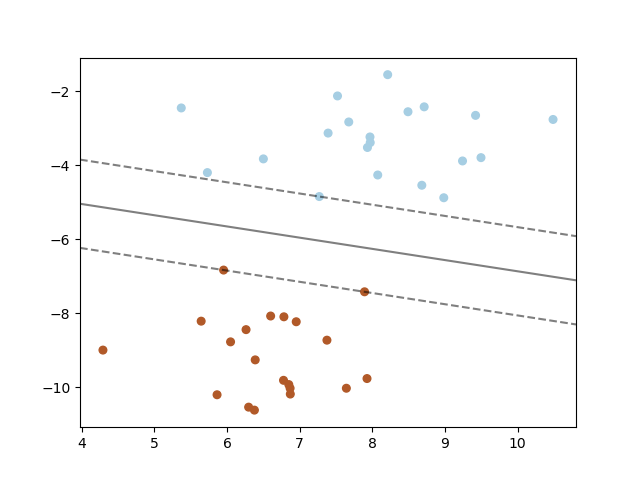
\includegraphics[width=0.5\textwidth]{images/svm_hiperplane}%
  \caption{La propagación y persistencia a través de paisajes heterogéneos}\label{fig:svm}
  \end{figure}

  Una SVM \cite{first_svm} construye un hiperplano o un conjunto de hiperplanos en un espacio
  de muy alta, o infinta, dimensionalidad. Éstos pueden ser usados tanto para
  tareas de regresión como de clasifición. Intuitivamente, una buena separación
  se consigue por el hiperplano que tenga la mayor distancia a los puntos de
  entrenamiento más cercanos de alguna clase, como bien se ve en la
  Figura \ref{fig:svm}, dado que en general
  a más grande sea esa distancia más pequeño será el error de generalización del
  modelo.

  Una Support Vector Regression VEEER (SVR) es una veloz y precisa forma de
  interpolación de conjuntos de datos. Es útil cuando se quiere aproximar sobre
  un dominio conocido una función costosa de calcular. Aprende rápidamente y
  se puede mejorar sistemáticamente.

  SVR es una generalización de la SVM a problemas de regresión. Tecnicamente,
  se puede decir que es un algoritmo de aprendizaje supervisado. Éste
  requiere de un conjunto de datos de entrenamiento,
  $\mathcal{T} = (\vec{X}, \vec{Y})$, que cubre el dominio de interés acompañado
  de las soluciones en dicho dominio. El trabajo de la SVM es aproximar la función
  definida por el conjnuto de entrenamiento, $F(\vec{X}) = \vec{Y}$. En general,
  en las SVM, los vectores $\vec{X}$ son utilizados para definir el hiperplano que
  separa las distintas soluciones posibles. En problemas de regresión, estos
  vectores son utilizados para realizar una regresión lineal, los que estén
  más cerca del punto de prueba se los llama \textit{vectores de soporte}.

  Daremos una idea más detallada de los fundamentos matemáticos detrás de una
  SVR \cite{svr_tutorial}:

  Dados los vectores de entrenamiento $x_{i} \in \mathbb{R}^{p}$ con $i = 1, \dots ,n$
  y un vector $y \in \mathbb{R}$ el $\epsilon$-SVR resuelve el siguiente problema
  primario:

  \begin{align}
    \min\limits_{w, b, \zeta, \zeta^{*}} \frac{1}{2} w^{T} w + C \sum_{i = 1}^{n} \zeta_{i}
  \end{align}
  con las restricciones de:


  \begin{math}
    y_{i} - w^{T} \phi(x_{i}) - b \leq \epsilon + \zeta_{i}, \\
    w^{T} \phi(x_{i}) + b - y_{i} \leq \epsilon + \zeta^{*}_{i}, \\
          \zeta^{*}_{i}, \zeta_{i} \geq 0 \\
    para\ i\ =\ 1,\ \dots, n
  \end{math}

  Mientras que el problema dual a resolver es:

  \begin{align}
    \min\limits{\alpha, \alpha^{*}} \frac{1}{2} (\alpha - \alpha^{*})^{T}
    Q(\alpha - \alpha^{*}) + \epsilon e^{T} (\alpha + \alpha^{*}) -
    y^{T} (\alpha - \alpha^{*})
  \end{align}
  con las restricciones de:

  \begin{math}
    e^{T} (\alpha - \alpha^{*}) = 0, \\
    0 \geq \alpha, \alpha^{*} \leq C \\
    para\ i\ =\ 1, \dots, n
  \end{math}

  Donde $e$ es un vector con todos sus componentes poseen el valor $1$, $C > 0$
  es la cota superior, $Q$ es una matriz semidefinida
  positiva\footnote{Una matriz, $M$, es semidefinida positiva si $x^{*}Mx \leq 0$
  $\forall x \in \mathbb{R}^{n}$} de tamaño $n \times n$,
  $Q_{ij} \equiv K(x_{i}, x_{j}) = \phi(x_{i}^{T})\phi(x_{j})$ es el núcleo
  (kernel, en inglés). Aquí, los vectores de entrenamiento están siendo mapeados
  un espacio de gran (probablemente infinita) dimensionalidad por la función
  $\phi$.
  Luego, la función de decisión es:
  \begin{align}
    \sum_{i = 1}^{n} (\alpha - \alpha^{*})K(x_{i}, x) + \rho
  \end{align}

\subsection{Perceptron Multicapa (MLP)}


\subsubsection{Fundamentos Matemáticos}
Dados ejemplos de entrenamiento $(x_{1}, y_{1}), \dots, (x_{n}, y_{n})$
donde $x_{i} \in \mathbb{R}^{n}$ y $y_{i} \in \{0,1\}$, un MLP de una capa oculta
de una neurona aprende una función $f(x) = W_{2}g(W_{1}^{T} x + b_{1}) + b_{2}$
donde $W_{1} \in \mathbb{R}^{m}$ y $W_{2}, b_{1}, b_{2} \in \mathbb{R}$ son
parametros del modelo.


\end{document}
